	
	1. Le tableau des chaudières :
	
	\[
\begin{array}{|c|c|c|c|}
	\hline
	\text{Type de chaudière} & \text{Défectueuse} & \text{Non défectueuse} & \text{Total} \\
	\hline
	\text{Cheminée} & 9 & 891 & 900 \\
		\hline
		\text{Ventouse} & 36 & 564 & 600 \\
	\hline
	\text{Total} & 45 & 1455 & 1500 \\
	\hline
\end{array}
	\]
	
	2. \begin{center}
		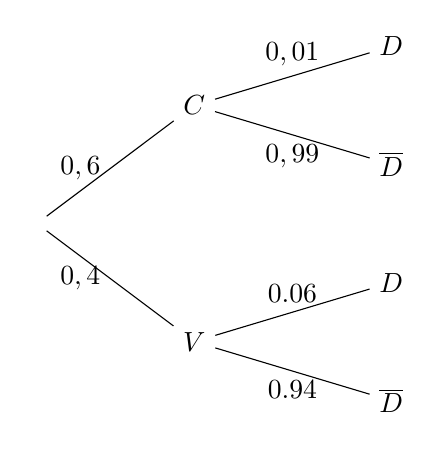
\begin{tikzpicture}
			[level 1/.style={level distance=2cm,
				sibling distance=3cm},
			level 2/.style={level distance=2.5cm,
				sibling distance=1.5cm}]
			\node {} [grow'=right]
			child {node {$C$}
				child {node {$D$}
					edge from parent node[above] {$0,01$}
				}
				child {node {$\overline D$}
					edge from parent node[below] {$0,99$}
				}
				edge from parent node[left] {$0,6$}
			}
			child {node {$ V$}
				child {node {$D$}
					edge from parent node[above] {$0.06$}
				}
				child {node {$\overline D$}
					edge from parent node[below] {$0.94$}
				}
				edge from parent node[left] {$0,4$}
			}
			;
		\end{tikzpicture}
	\end{center}
	3.
	\[
	\begin{aligned}
		P(C \cap D) &= P(C) \times P_C(D) = 0,6 \times 0,01 = 0,006, \\
		P(V \cap D) &= P(V) \times P_V(D) = 0,4 \times 0,06 = 0,024, \\
		P(D) &= P(C \cap D) + P(V \cap D) = 0,006 + 0,024 = 0,03.
	\end{aligned}
	\]
	
	4. On a :
	\[
	P_D(V) = \dfrac{P(D \cap V)}{P(D)} = \dfrac{0,024}{0,03} = 0,8.
	\]
	80\% des chaudières défectueuses sont à ventouses.
	
	5. Puisque $P(V) \times P(D) \neq P(V \cap D)$, les événements $D$ et $V$ ne sont pas indépendants.
	
